\documentclass[twoside]{article}
\usepackage{mdframed}
\usepackage[hmarginratio=1:1,top=32mm,columnsep=20pt]{geometry} % Document margins
\usepackage{multicol} % Used for the two-column layout of the document
\usepackage[hang, small,labelfont=bf,up,textfont=it,up]{caption} % Custom captions under/above floats in tables or figures
\usepackage{booktabs} % Horizontal rules in tables
\usepackage{float} % Required for tables and figures in the multi-column environment - they need to be placed in specific locations with the [H] (e.g. \begin{table}[H])
\usepackage{hyperref} % For hyperlinks in the PDF
\usepackage{amsmath,amsthm,amssymb}
\usepackage{lettrine} % The lettrine is the first enlarged letter at the beginning of the text
\usepackage{paralist} % Used for the compactitem environment which makes bullet points with less space between them
\usepackage{tikz}
\usepackage{esint}
\usepackage{centernot}
\usepackage{lmodern}
\usetikzlibrary{3d}
\usetikzlibrary{patterns,calc,hobby}
\usetikzlibrary{decorations.pathreplacing}
\tikzset{
	partial ellipse/.style args={#1:#2:#3}{
		insert path={+ (#1:#3) arc (#1:#2:#3)}
	}
}
\usepackage{xcolor}

\usepackage{fancyhdr} % Headers and footers
\pagestyle{fancy} % All pages have headers and footers
\fancyhead{} % Blank out the default header
\fancyfoot{} % Blank out the default footer
\fancyhead[C]{Jimmy Yue $\bullet$ Statistics $\bullet$ Jimmy Yue} % Custom header text
\fancyfoot[RO,LE]{\thepage} % Custom footer text

\newmdenv[skipabove=7pt,
rightline=false,
leftline=true,
topline=false,
bottomline=false,
skipbelow=5pt,
linecolor=black,
innerleftmargin=5pt,
innerrightmargin=5pt,
innertopmargin=5pt,
leftmargin=0cm,
rightmargin=0cm,
linewidth=4pt,
innerbottommargin=5pt]{cBox}

\theoremstyle{definition}
\newtheorem*{solutionT}{Solution}

\newenvironment{solution}{\begin{cBox}\begin{solutionT}}{\hfill{\scriptsize\ensuremath{\square}}\end{solutionT}\end{cBox}}

%%%%%%%%%%%%%%%%%%%%%%%%%%%%%%%%%%%%%%%%%%%%%%%%%%%%%%%%%%%%%%%%%%%%%%%%%%%%%%%%%%%%%%%%%%%%
\newcommand{\vect}[1]{\vec{\pmb{#1}}}
\newcommand{\uvect}[1]{\hat{\mathbf{#1}}}
\newcommand{\leviciv}{\epsilon_{ijk}}

\newmdenv[skipabove=7pt,
rightline=false,
leftline=true,
topline=false,
bottomline=false,
skipbelow=5pt,
linecolor=black,
innerleftmargin=5pt,
innerrightmargin=5pt,
innertopmargin=5pt,
leftmargin=0cm,
rightmargin=0cm,
linewidth=4pt,
innerbottommargin=7,
backgroundcolor=light-gray]{dBox}



\theoremstyle{definition}
\newtheorem*{proof1}{Definition}

\newenvironment{ddef}{\begin{dBox}\begin{proof1}}{\hfill{\scriptsize}\end{proof1}\end{dBox}}
\newcommand{\pdif}[2]{\frac{\partial#1}{\partial#2}}
\definecolor{light-gray}{gray}{0.85}
%----------------------------------------------------------------------------------------
%-	TITLE SECTION
%----------------------------------------------------------------------------------------

\title{\vspace{-15mm}\fontsize{24pt}{10pt}\selectfont\textbf{Statistics - Week 2}} % Article title

\author{
\large
\textsc{Jimmy Tsz Ming Yue}\thanks{440159151}\\[2mm] % Your name
\normalsize University of Sydney \\ % Your institution
\normalsize \href{mailto:jyue6728@uni.sydney.edu.au}{jyue6728@uni.sydney.edu.au} % Your email address
\vspace{-5mm}
}
\date{}

%----------------------------------------------------------------------------------------

\usepackage{Sweave}
\begin{document}
\Sconcordance{concordance:w2.tex:w2.Rnw:%
1 210 1 1 2 1 0 1 1 3 0 1 2 3 1 1 2 4 0 1 2 1 1 1 2 7 0 1 2 5 1 1 2 9 0 %
1 11 6 0 1 2 8 1 1 8 7 0 1 1 3 0 2 2 1 0 1 1 3 0 2 2 5 0 1 2 8 1 1 2 1 %
0 1 1 1 2 1 0 1 1 32 0 1 2 3 1}

\maketitle % Insert title

\thispagestyle{fancy} % All pages have headers and footers
\hrule \smallskip

\noindent Semester 2 \quad Statistics \hspace{11.5
cm} 2018
\smallskip
\hrule
\smallskip
\tableofcontents
\section{What is clustering?}

\begin{ddef}
	Clustering are methods of grouping samples $(x)$ that are similar in nature, according to some pre-defined criteria. It is a form of unsupervised learning, in that there is no label information $(y)$ to tell the algorithm which observations should be grouped together. As such it is often used for exploratory data analysis: for which we can look at patters or structures in the data set which may be of particular interest to us. 
\end{ddef}
\section{Basic Principles of Clustering}

In clustering, we aim to group observations that are similar. There are certain issues that arise from this , which include consideration of the data types, the prescence of missing data, scaling and the similarity metric that we chose in doing our clustering. Examples of such metrics are: Euclidean, Manhattan, Pearson correlation, Spearman correlation. To do clustering we can employ many different algorithms, such as: Hierarchical clustering, K-means clustering, Fuzzy c-means clustering, semi-supervised clustering and bi-clustering.

\section{Commonly used similarity measures}

\begin{ddef}
	\textbf{Metric}: A metric is a measure of the similarity or dissimilarity between two data objects and it is used to form data points into cluster. (Formally speaking a metric is a measure of the distance within a metric space). We have:

	\begin{enumerate}
		\item Correlation Coefficients, which compares the shape of expression curves; (Pearson's Correlation Coefficient):
			\begin{align}
				\rho(x,y) & = \frac{\sum^n_{i=1}(x_i-\bar{x})(y_i-\bar{y})}{\sqrt{\sum^n_{i=1}(x_i-\bar{x})^2}\sqrt{\sum^n_{i=1}(y_i-\bar{y})^2}}\\
				d_p & = \frac{1-\rho(x,y)}{2}
			\end{align}
		\item Distance Metrics, where we have; 
			\begin{enumerate}
				\item Manhattan distance;

					\begin{align*}
						d(X,Y) = \sum_i|x_i - y_i|
					\end{align*}
				\item Euclidean distance;
					\begin{align*}
					d(x,y) = \sqrt{\sum^n_{i=1} (x_i - y_i)^2}
				\end{align*}
			\end{enumerate}

	\end{enumerate}
	We also have Spearman's and Kendall's correlation which we can use to define our metrics. We can use absolute correlation to capture both positive and negative correlation. 
\end{ddef}
\section{Distances between clusters}
We can choose different measures for measuring between clusters, with:
\begin{enumerate}
	\item Single: Which measures the closest distance between two clusters
	\item Complete: Which measures the maximum distance between two clusters
	\item Distance between centroids, which measures between the centroid of two clusters
	\item Average Linkage: Which takes the average distance between clusters. 
\end{enumerate}
\section{Clustering Algorithms}
We have two different flavours of clusterings;
\begin{enumerate}
	\item Partitioning
	\item Hierarchical
\end{enumerate}

\subsection{Hierarchical methods}
Hierarchical clustering methods produce a tree or dendrogram. They avoid specifying how many clusters are approrpriate by providing a partition for each $k$ obtained from cutting the tree at some level. An example of hierarchical clustering is the bottom-up tree buidling. This is done as follows:

\begin{dBox}
	\textbf{Bottom-Up Tree building procedure}
	\begin{enumerate}
		\item Let us start with $n$ samples for which we generate $n$ clusters.
		\item At each step, we merge the two closest clusters using a measure of between-cluster dissimilarity which reflects the shape of the clusters. (We may use different measures of distance as outlined above) 
	\end{enumerate}
\end{dBox}

Let us give some examples first with some R code of the crime data given last week then with Gene expression data;

\begin{cBox}
	
\end{cBox}

\begin{cBox}
	
\end{cBox}

\subsection{Partitioning methods}
Partitioning clustering methods seeks to partition the data into pre-specified number $k$ of mutually exclusive and exhuastive groups. This is done through iteratively reallocating the observations to clusters until some critierion is met, for example the minimisation of cluster sums of squares. 

\begin{dBox}
	\textbf{Typical Clustering Algorithm}
	\begin{enumerate}
		\item Choose $k$ objects as the initial cluster centers
		\item Until no change, 
		\item Reassign each object to the cluster to which the object is the most similar, based on the mean value of the objects in the cluster.
		\item Update the cluster means, 
	\end{enumerate}
\end{dBox}

\subsubsection{Problems with $k$-means}
There are some issues with paritioning, namely the prescence of outliers. For example, objects with extremely large values may substantially distort the distribution of data. 

\section{Tutorial 2}

The "ClueR" R package contains a time-course phosphoproteomics dataset "hES". Each
column of in hES data is a time point and each row is a phosphorylation sites. We will
perform clustering analysis on this dataset.

\begin{enumerate}
  \item Install “ClueR” R package and its dependent packages. Find out how to use it by
typing “?runClue”.
\begin{solution}
Let us load the library:
\begin{Schunk}
\begin{Sinput}
> library("ClueR")
> ?runClue
\end{Sinput}
\end{Schunk}

\end{solution}
\item Once you have installed the package load the hES dataset as follows:

\begin{Schunk}
\begin{Sinput}
> data(hES)
\end{Sinput}
\end{Schunk}
\begin{solution}
Find out the dimension of the hES dataset.
\begin{Schunk}
\begin{Sinput}
> dim(hES)
\end{Sinput}
\begin{Soutput}
[1] 3416    5
\end{Soutput}
\end{Schunk}
\end{solution}

\item Create hierarchical clustering with respect to times (i.e. cluster the columns). How
does time points cluster with each other? Does it make sense?
\begin{solution}
Let us have a look at the dataset to generate some perspective:
\begin{Schunk}
\begin{Soutput}
            0        30m        1hr       6hrs      24hrs
SFRS4;118;  0  0.5753123  0.6229304  0.5058909 -1.1844246
SFRS4;119;  0  0.5753123  0.7224660  0.5058909 -1.1844246
PPP2R5D;88; 0 -0.6665763 -1.3219281 -0.3219281  0.4329594
PPP2R5D;89; 0 -0.6214884 -1.4344028 -0.2688168  0.2986583
PPP2R5D;90; 0 -0.6214884 -1.4344028 -0.4150375  0.2986583
PPP2R5D;95; 0 -0.6214884 -1.4344028 -0.3219281  0.2986583
\end{Soutput}
\begin{Soutput}
hc.clusters
   1    2    3    4    5 
2121 1247   40    5    3 
\end{Soutput}
\end{Schunk}
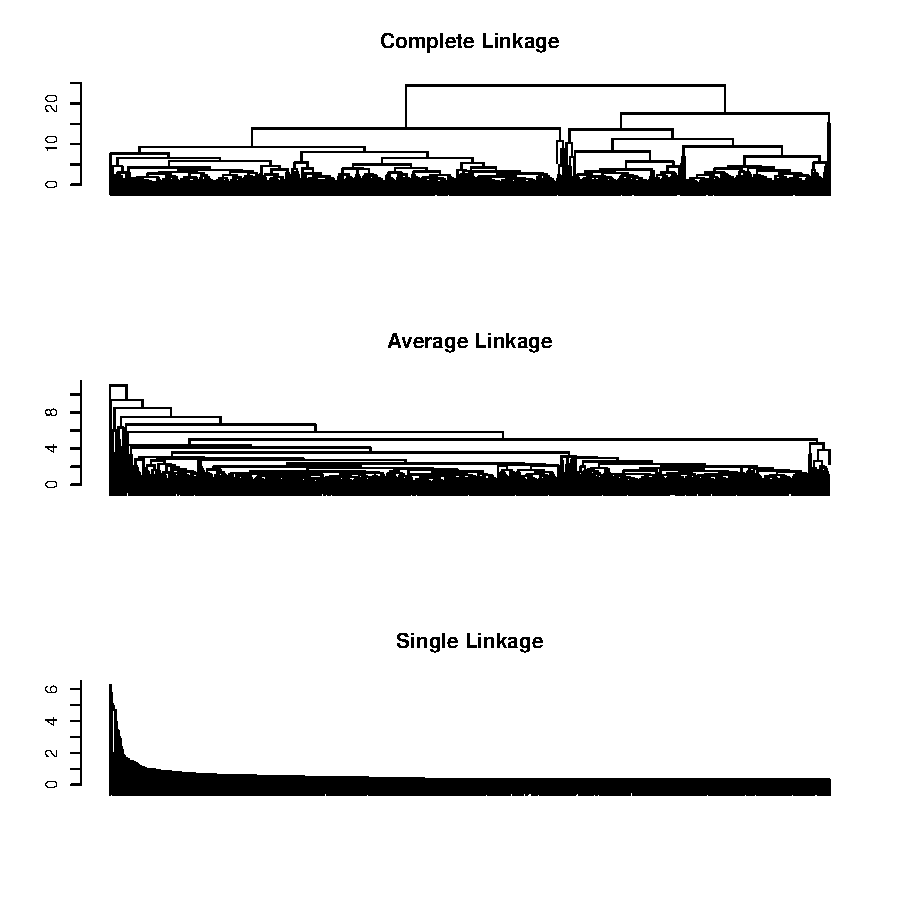
\includegraphics{w2-004}
\begin{cBox}
NB the t() function returns the transpose of a matrix
\end{cBox}
\end{solution}

\item Install package “e1071” and apply c-means clustering to partition the data in to 9
groups ($c=9$) with respect to phosphorylation sites (i.e. partition rows into c groups).
Firstly, standardise the data to be unit free.

\begin{Schunk}
\begin{Sinput}
> standardize <- function(mat) {
+ means <- apply(mat, 1, mean)
+ stds <- apply(mat, 1, sd)
+ tmp <- sweep(mat, 1, means, FUN="-")
+ mat.stand <- sweep(tmp, 1, stds, FUN="/")
+ return(mat.stand)
+ }
> hES.scaled <- standardize(hES)
\end{Sinput}
\end{Schunk}
Once the data is standardised the data to be unit free, perform clustering.
\begin{Schunk}
\begin{Sinput}
> library(e1071)
> fc <- cmeans(hES.scaled, centers=9)
\end{Sinput}
\end{Schunk}
Visualise the clustering results using ClueR package function “fuzzPlot” as follows:
\begin{Schunk}
\begin{Sinput}
> fuzzPlot(hES.scaled, fc, mfrow = c(3, 3))
\end{Sinput}
\end{Schunk}
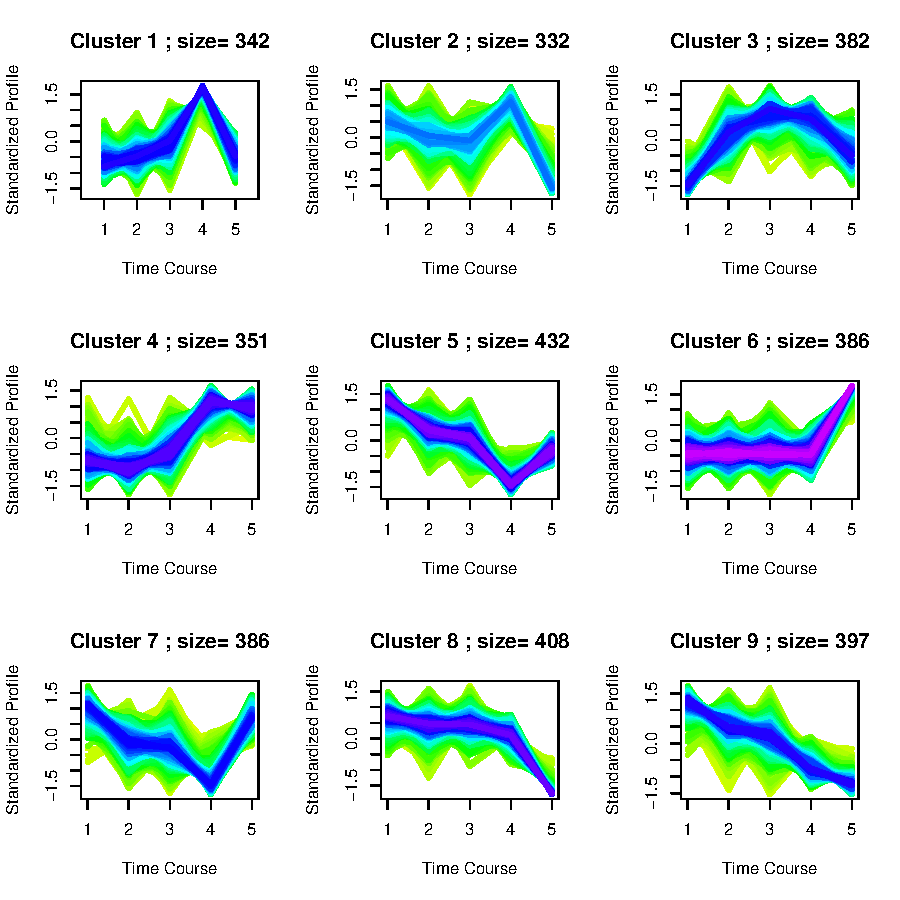
\includegraphics{w2-007}

\begin{solution}
\end{solution}
\item Is $k=9$ the best choice of k? Apply Dunn index to validate k-means clustering using
different k values. Which K gives best clustering results according to Dunn index?
Does it differ if we use other validation index such as Connectivity or APN?
\begin{solution}
Let us quickly generate the dunn index for the dataset for differing k values:

\begin{Schunk}
\begin{Sinput}
> library(cluster)
> library(clValid)
> intern <- clValid(hES.scaled, nClust=2:9, validation=c("internal", "stability"), 
+ clMethods="kmeans", maxitems=nrow(hES.scaled))
> summary(intern)
\end{Sinput}
\begin{Soutput}
Clustering Methods:
 kmeans 

Cluster sizes:
 2 3 4 5 6 7 8 9 

Validation Measures:
                            2        3        4        5        6        7        8        9
                                                                                            
kmeans APN             0.2125   0.2323   0.2781   0.3804   0.3788   0.3941   0.4789   0.4774
       AD              2.3322   2.0901   1.9332   1.9398   1.8315   1.7491   1.7392   1.7008
       ADM             0.6133   0.5991   0.6283   0.8393   0.7811   0.7722   0.9256   0.9159
       FOM             0.8531   0.8155   0.7979   0.7923   0.7354   0.7176   0.7167   0.6926
       Connectivity  210.3500 332.8917 395.2639 427.1460 495.8353 516.9726 576.8060 639.4250
       Dunn            0.0289   0.0158   0.0246   0.0037   0.0121   0.0130   0.0159   0.0253
       Silhouette      0.3086   0.2974   0.2833   0.2893   0.2932   0.3041   0.2768   0.2685

Optimal Scores:

             Score    Method Clusters
APN            0.2125 kmeans 2       
AD             1.7008 kmeans 9       
ADM            0.5991 kmeans 3       
FOM            0.6926 kmeans 9       
Connectivity 210.3500 kmeans 2       
Dunn           0.0289 kmeans 2       
Silhouette     0.3086 kmeans 2       
\end{Soutput}
\end{Schunk}
As we can see, in Dunn Index, Silhouette and APN, the optimal score is 2 clusters.  (We recall that Dunn index is between $[0,\infty)$) and should be maximised. In contrast connectivity should be miniised with APN between 0 and 1 and minimial values indicating consistent clustering.
\end{solution}
\end{enumerate}
\end{document}
